\documentclass[10pt,table,dvipsnames]{beamer}

\usepackage{tikz}
\usepackage[absolute,overlay]{textpos}

\author{C.~Grefe, S.~Poss, A.~Sailer}
\title{ILCDIRAC}
\subtitle{A grid solution for the LC community}
\date{Oct. 1st 2013, CLIC dp meeting}
\institute{CERN}
\newcommand{\interstitial}[1]{\begin{frame}\begin{block}{}\centering\Huge{#1}\end{block} \end{frame}}
\newcommand{\backupslides}{\interstitial{Backup Slides}}

\mode<all>
\TPGrid{50}{50}

\pgfdeclareimage[width=0.1\paperwidth]{cliclogo}{CLIClogo}
\newcommand{\ClicLogo}{%
\begin{textblock}{14}(45., 0.05)
 \href{http://lcd.web.cern.ch}{\pgfuseimage{cliclogo}}
\end{textblock}
}

\setbeamertemplate{footline}
{%
  \leavevmode%
  \hbox{%
  \begin{beamercolorbox}[wd=.222222\paperwidth,ht=2.25ex,dp=1ex,left]{title in 
head/foot}%
    \usebeamerfont{date in head/foot}\insertshortdate{}\hspace*{2em}
  \end{beamercolorbox}%
  \begin{beamercolorbox}[wd=.555555\paperwidth,ht=2.25ex,dp=1ex,center]{author 
in head/foot}%
    \usebeamerfont{author in head/foot}\insertshortauthor{}:
    \usebeamerfont{title in head/foot}\insertshorttitle
  \end{beamercolorbox}%
  \begin{beamercolorbox}[wd=.222222\paperwidth,ht=2.25ex,dp=1ex,right]{date in 
head/foot}%
    \insertframenumber{}/\inserttotalframenumber\hspace*{2ex}
  \end{beamercolorbox}}%
  %\vskip0pt%
  \ClicLogo
}
\beamertemplatenavigationsymbolsempty 
\setbeamertemplate{blocks}[rectangle]
\setbeamersize{text margin left=1em,text margin right=1em}

%\setbeamertemplate{headline}[default]

\begin{document}
\renewcommand{\inserttotalframenumber}{\ref{lastframe}}
\begin{frame}
\titlepage
\end{frame}

\begin{frame}
\frametitle{Outline}
\tableofcontents
\end{frame}

\section{Current status}
\begin{frame}
\frametitle{Current status}
ILCDIRAC now stable, no more developments, only bug fixes.

~\\

ILD concept now moves towards using DIRAC:
\begin{itemize}
\item Several questions came
\item ILCDIRAC required a few fixes to adapt to that use case: Production job class, support for application specific inputs (ILDConfig package)
\item File Catalog meta data adjustements for ILD
\item The web interface to the File Catalog has issues, but working on those now. Next major version of the portal will have a different interface.
\end{itemize}
~\\
More users are coming every week, now $\approx 100$ registered, 20 active
\end{frame}

\begin{frame}
\frametitle{Current status}
\centering
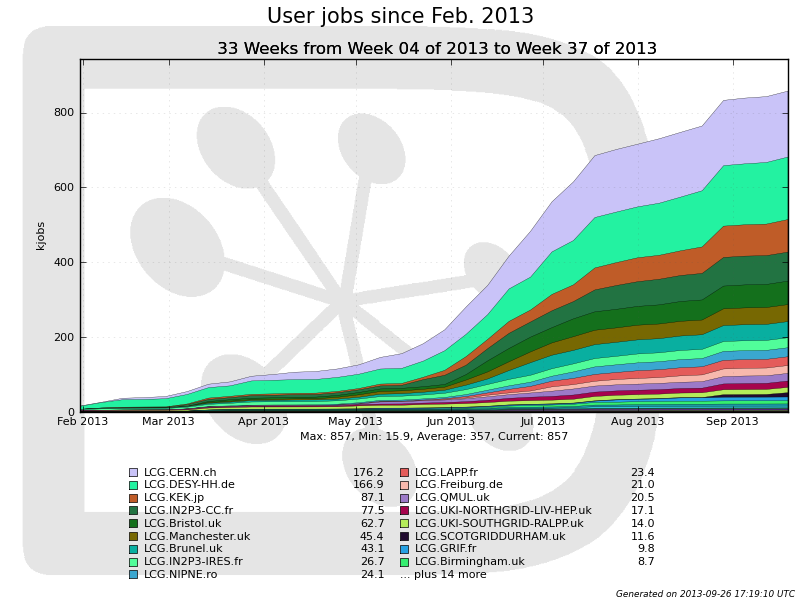
\includegraphics[width=0.9\textwidth]{userjobs}
\end{frame}
\begin{frame}
\frametitle{Current status}
\centering
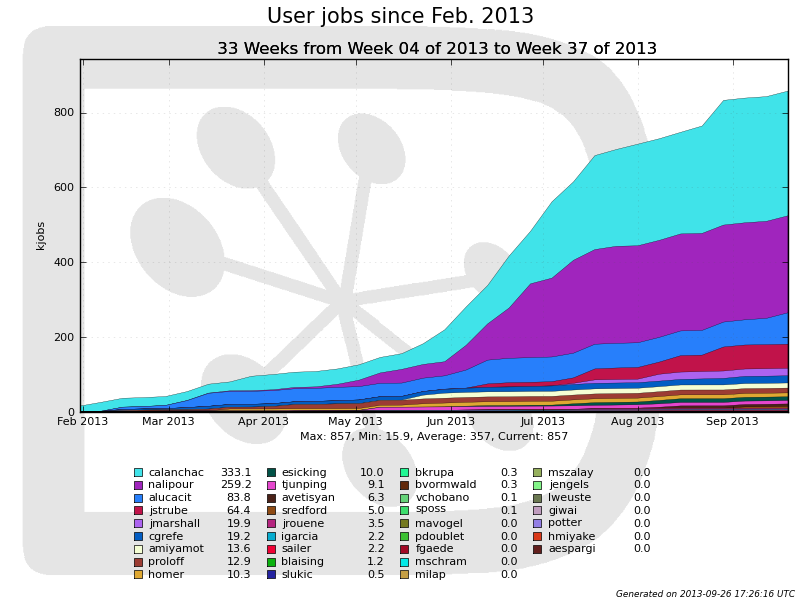
\includegraphics[width=0.9\textwidth]{userjobsperuser}
\end{frame}
\begin{frame}
\frametitle{Current status}
\centering
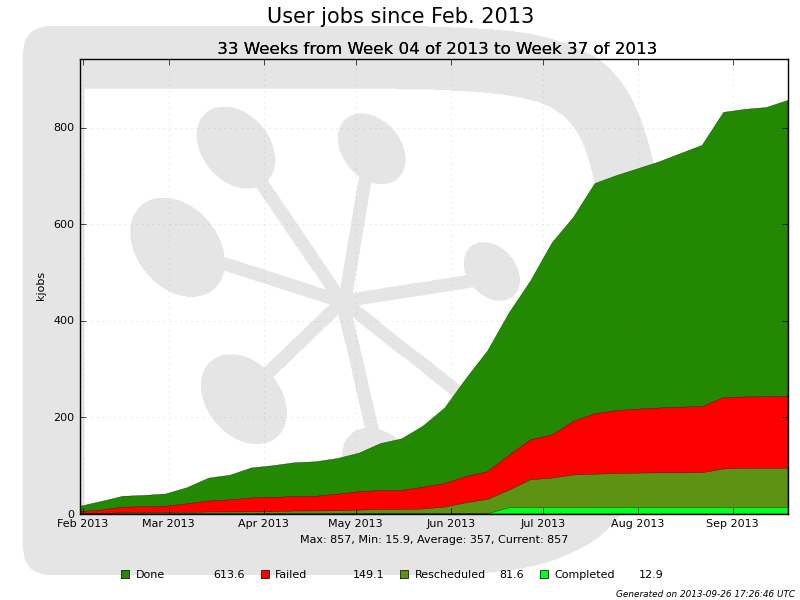
\includegraphics[width=0.9\textwidth]{userjobsperstatus}
\end{frame}

\begin{frame} 
\frametitle{Current status}
\centering
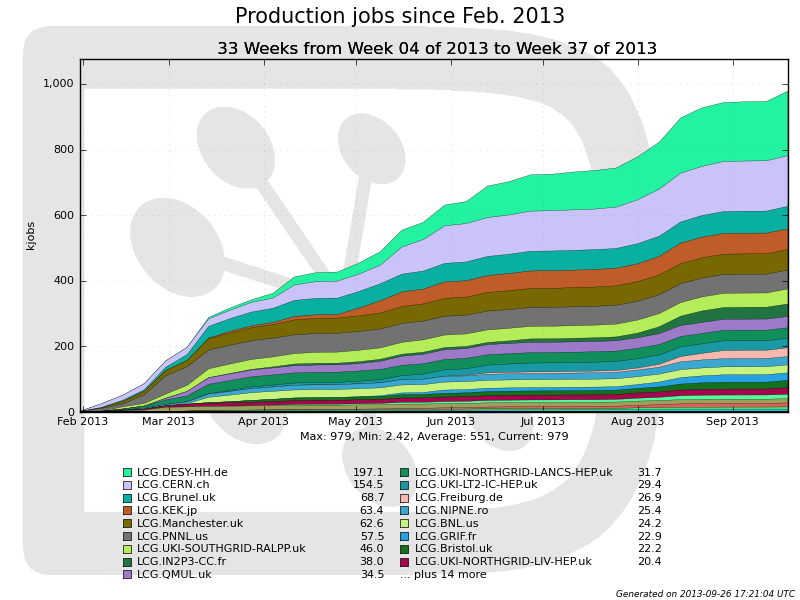
\includegraphics[width=0.9\textwidth]{prodjobs}
\end{frame} 

\section{File catalog}
\begin{frame}
\frametitle{DIRAC File Catalog}
The file catalog includes most files produced for the ILC DBD, all files 
for the SID DBD, all files for CLIC. LFC and DFC are written in parallel, and
thanks to the failover mechanism: \alert{NO DATA LOSS}

~\\

Top 5 disk usage {\scriptsize (FC:/$>$size -l)}:\\
\begin{center}
\begin{tabular}{|ccccc|}
\hline
Storage & Disk use & CLIC & ILC & Replicas \\
\hline
CERN-SRM & 868 TB & 861 TB & 7 TB & 4\,053\,817\\
\hline
DESY & 96 TB & 0 & 96 TB& 306\,585\\
\hline
KEK & 95 TB & 76 GB & 94 TB & 244\,148\\
\hline
RAL-SRM & 93 TB & 4TB & 89 TB & 1\,026\,781\\
\hline
PNNL-SRM & 25 TB & 0 & 25 TB & 733\,423\\
\hline
\end{tabular}
\end{center}
Most data produced for the CLIC CDR.

\end{frame}

\section{Bug tracking}
\begin{frame}
\frametitle{Bug tracking}
Use of JIRA: http://its.cern.ch/jira/browse/ILCDIRAC
\begin{center}
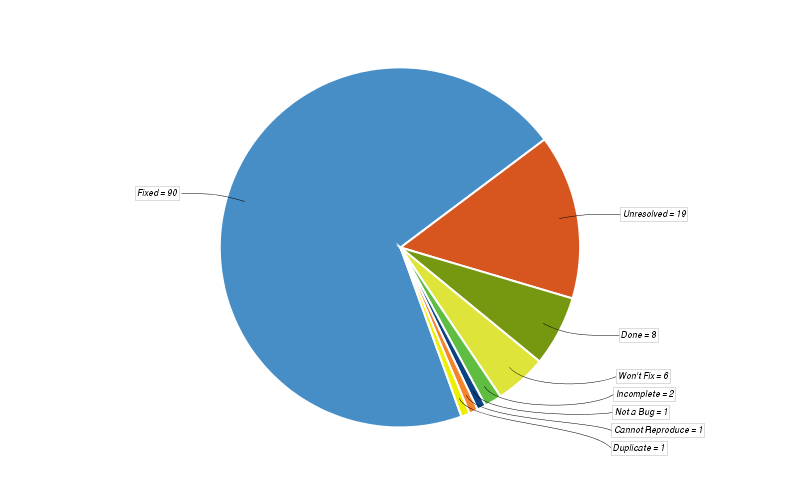
\includegraphics[width=0.8\textwidth]{charts_1}
\end{center}
\end{frame}
\begin{frame}
\frametitle{Bug tracking}
From Web portal:
\centering
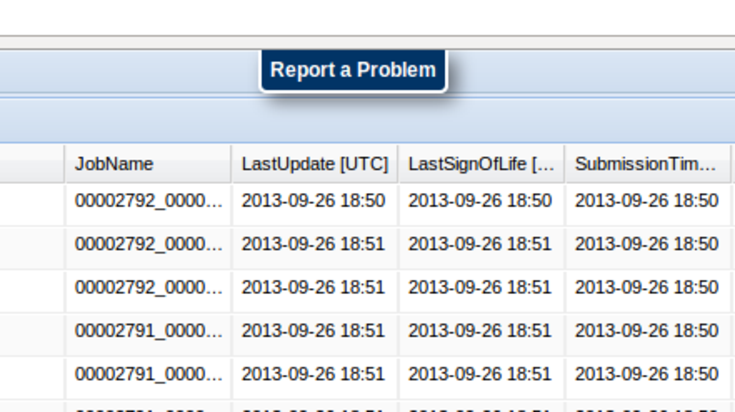
\includegraphics[width=0.9\textwidth]{ReportProb} 
\end{frame}

\section{Contact info}
\begin{frame}
\frametitle{Mailing lists}
Register: ilcdirac-register@cern.ch

~\\

Questions: ilcdirac-support@cern.ch

~\\

Forum:\\ 
\scriptsize \url{http://forum.linearcollider.org/index.php?t=index&cat=22&rid=0&S=e56e5487e1f220b0b5f4a425989fcbd7}
\vfill
\begin{center}
\alert{\Large Any new user is welcome!}
\end{center}

\label{lastframe}
\end{frame} 
 

\end{document}


% Local Variables:
% TeX-PDF-mode: t
% End:
